\documentclass{standalone}

\usepackage{tikz}
    \usetikzlibrary{arrows.meta}
    
\begin{document}
\begin{tikzpicture}
    % \draw[help lines] (0,0) grid (11,5);
    \node at (5,5) {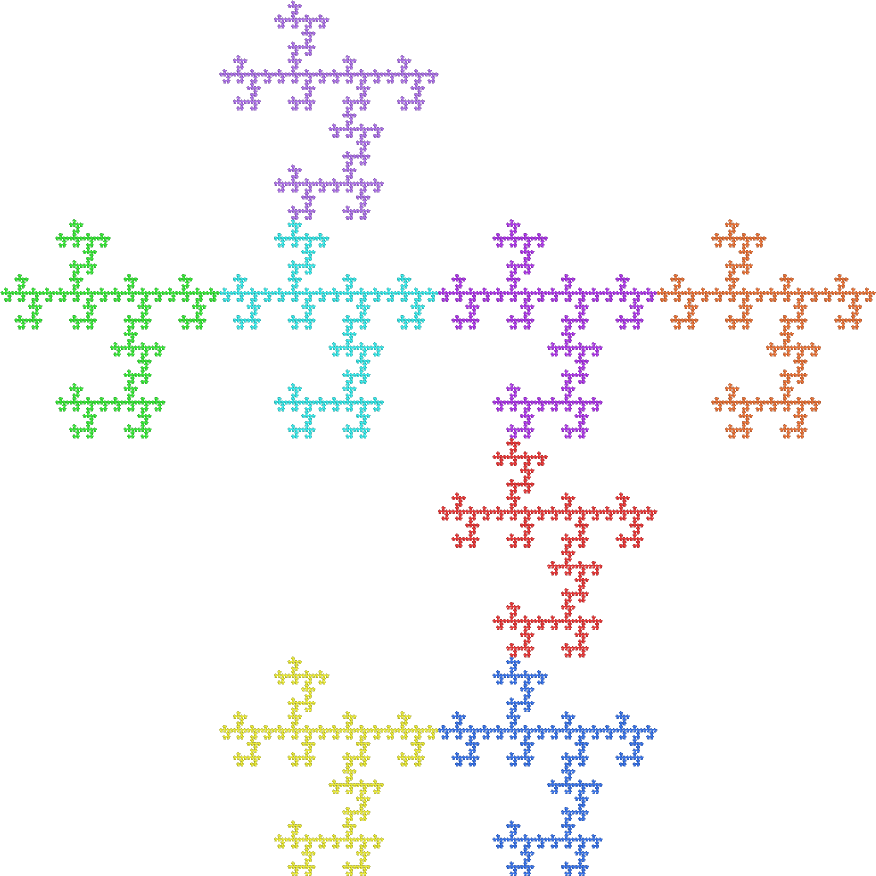
\includegraphics[width=10cm]{A-type.png}};
    \foreach \x in
        {(0,6.66), (10,6.66), (3.33,0), (3.33,10)} 
        {\fill \x circle(0.15);}
    \path[->,>={Latex[length=5mm]}, line width=1mm, red]
        (-1,6.66) edge (0,6.66)
        (11,6.66) edge (10,6.66);
    \path[->,>={Latex[length=5mm]}, line width=1mm, black]
        (3.33,-1) edge (3.33,0)
        (3.33,11) edge (3.33,10);
\end{tikzpicture}
\end{document}